Sikteeri on Kapsi ry:n laskutuksen ja jäsenhallinnan tarpeisiin kehitetty web-palvelu. Sikteeriin on pääsy Kapsi ry:n hallituksella, ylläpidolla ja ryhmään laskutus kuuluvilla jäsenillä. Lisäksi yhdistyksellä on käytössään erillinen komentorivityökalu, nimeltä admtool, jolla voidaan tehdä erilaisia ylläpitotehtäviä.

Sekä Sikteeri että admtool käyttävät ulkoisena komponenttina LDAP-käyt\-tä\-jä\-hal\-lin\-taa, josta tarkistetaan onko käyttäjällä oikeuksia käyttää kyseisiä palveluita. Nykyinen arkkitehtuuri on kuvattu kuvassa \ref{kapsi_nykyinen}. Kuvaan on lisätty myös suunnitteilla oleva käyttäjien palvelunhallinta, jota kautta jäsenet voisivat lisätä itselleen jäsenmaksuun kuuluvia palveluita, kuten sähköpostialiaksia ja domaineja. Myös käyttäjien palvelunhallinnan tarvitsee tunnistaa käyttäjät, joten nykyisessä arkkitehtuurissa myös sen täytyy integroitua LDAP-käyttäjänhallintaan.

\begin{figure}[h]
\centering
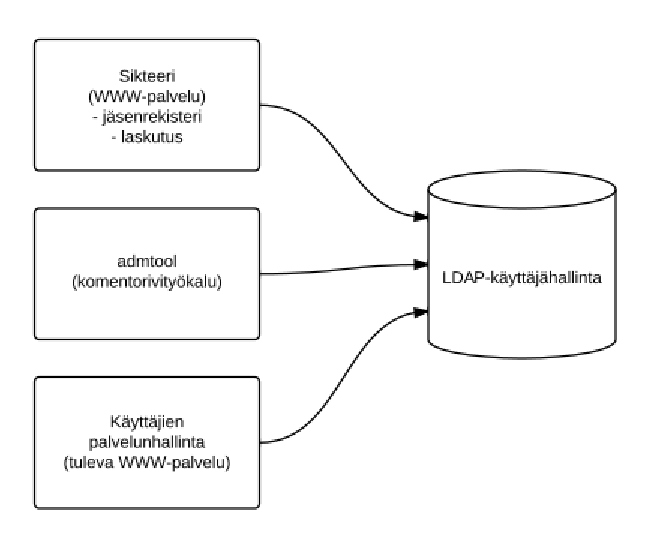
\includegraphics[width=.7\textwidth]{toteutus/kapsi_nykyinen.eps}
\caption{Kapsin jäsenhallintapalveluiden arkkitehtuuri.}%
\label{kapsi_nykyinen}
\end{figure}

Nykyisen arkkitehtuurin ongelma ovat useat integroinnin LDAP-palvelimeen. LDAP:in on talletettu jäsenten henkilökohtaista dataa, kuten henkilötunnus, joten tietoturvasyistä siihen halutaan integroida mahdollisimman vähän eri sovelluksia. Tällä hetkellä sovelluksia on vain Sikteeri ja admtool, mutta pidemmän aikavälin tavoitteena on uusien palveluiden (kuten käyttäjien palvelunhallinta) toteuttaminen sekä nykyisen Sikteerin jakaminen pienempiin osapalveluihin palvelusuuntautuneen arkkitehtuurin mukaisesti. Kuvassa \ref{kapsi_uusi} on esitetty tavoiteltu arkkitehtuuri, jossa Sikteerin laskutus- ja jäsenrekisteripalvelut on itsenäisiä web-sovelluksia ja joiden rinnalla on admtool-komentorivityökalu sekä käyttäjien palvelunhallinta. LDAP:n integraatiopisteiden määrä on yksi, sillä LDAP kommunikoi vain keskitetyn tunnistautumispalvelun kanssa, joka taas tarjoaa Kapsi ry:n web-sovelluksille tunnistautumisrajapinnat.

\begin{figure}[ht]
\centering
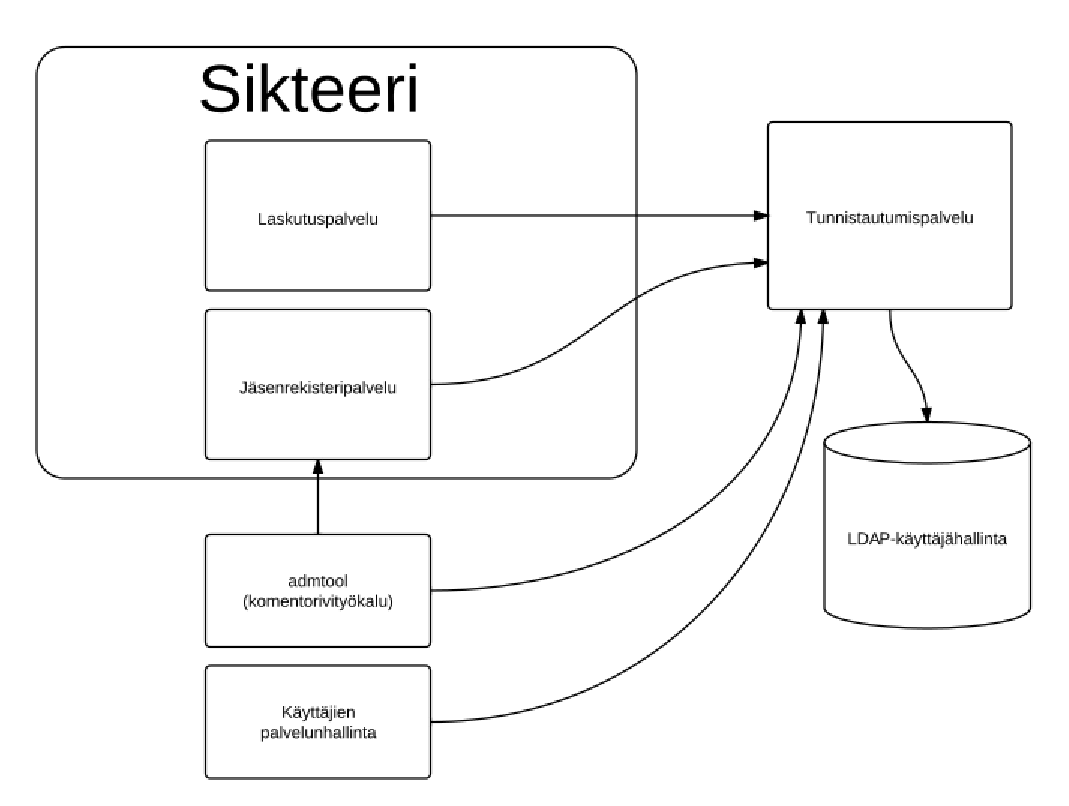
\includegraphics[width=.7\textwidth]{toteutus/kapsi_uusi.eps}
\caption{Palvelusuuntautuneen arkkitehtuurin mukainen kuvaus Kapsin järjestelmästä. Sikteerin palvelut on jaoteltu omiksi komponenteiksi ja järjestelmään on lisätty keskitetty tunnistautumispalvelu.}%
\label{kapsi_uusi}
\end{figure}

Tämän tutkielman kannalta oleellisin osa uudessa arkkitehtuurissa on keskitetyn tunnistautumispalvelun toteuttaminen. Sikteerin nykyinen toteutus ja suunniteltu jatkokehitys asettavat tiettyjä vaatimuksia toteutettavalle tunnistautumispalvelulle. Näitä vaatimuksia sekä muita reunaehtoja käsitellään seuraavassa alaluvussa.